\documentclass[1p]{elsarticle_modified}
%\bibliographystyle{elsarticle-num}

%\usepackage[colorlinks]{hyperref}
%\usepackage{abbrmath_seonhwa} %\Abb, \Ascr, \Acal ,\Abf, \Afrak
\usepackage{amsfonts}
\usepackage{amssymb}
\usepackage{amsmath}
\usepackage{amsthm}
\usepackage{scalefnt}
\usepackage{amsbsy}
\usepackage{kotex}
\usepackage{caption}
\usepackage{subfig}
\usepackage{color}
\usepackage{graphicx}
\usepackage{xcolor} %% white, black, red, green, blue, cyan, magenta, yellow
\usepackage{float}
\usepackage{setspace}
\usepackage{hyperref}

\usepackage{tikz}
\usetikzlibrary{arrows}

\usepackage{multirow}
\usepackage{array} % fixed length table
\usepackage{hhline}

%%%%%%%%%%%%%%%%%%%%%
\makeatletter
\renewcommand*\env@matrix[1][\arraystretch]{%
	\edef\arraystretch{#1}%
	\hskip -\arraycolsep
	\let\@ifnextchar\new@ifnextchar
	\array{*\c@MaxMatrixCols c}}
\makeatother %https://tex.stackexchange.com/questions/14071/how-can-i-increase-the-line-spacing-in-a-matrix
%%%%%%%%%%%%%%%

\usepackage[normalem]{ulem}

\newcommand{\msout}[1]{\ifmmode\text{\sout{\ensuremath{#1}}}\else\sout{#1}\fi}
%SOURCE: \msout is \stkout macro in https://tex.stackexchange.com/questions/20609/strikeout-in-math-mode

\newcommand{\cancel}[1]{
	\ifmmode
	{\color{red}\msout{#1}}
	\else
	{\color{red}\sout{#1}}
	\fi
}

\newcommand{\add}[1]{
	{\color{blue}\uwave{#1}}
}

\newcommand{\replace}[2]{
	\ifmmode
	{\color{red}\msout{#1}}{\color{blue}\uwave{#2}}
	\else
	{\color{red}\sout{#1}}{\color{blue}\uwave{#2}}
	\fi
}

\newcommand{\Sol}{\mathcal{S}} %segment
\newcommand{\D}{D} %diagram
\newcommand{\A}{\mathcal{A}} %arc


%%%%%%%%%%%%%%%%%%%%%%%%%%%%%5 test

\def\sl{\operatorname{\textup{SL}}(2,\Cbb)}
\def\psl{\operatorname{\textup{PSL}}(2,\Cbb)}
\def\quan{\mkern 1mu \triangleright \mkern 1mu}

\theoremstyle{definition}
\newtheorem{thm}{Theorem}[section]
\newtheorem{prop}[thm]{Proposition}
\newtheorem{lem}[thm]{Lemma}
\newtheorem{ques}[thm]{Question}
\newtheorem{cor}[thm]{Corollary}
\newtheorem{defn}[thm]{Definition}
\newtheorem{exam}[thm]{Example}
\newtheorem{rmk}[thm]{Remark}
\newtheorem{alg}[thm]{Algorithm}

\newcommand{\I}{\sqrt{-1}}
\begin{document}

%\begin{frontmatter}
%
%\title{Boundary parabolic representations of knots up to 8 crossings}
%
%%% Group authors per affiliation:
%\author{Yunhi Cho} 
%\address{Department of Mathematics, University of Seoul, Seoul, Korea}
%\ead{yhcho@uos.ac.kr}
%
%
%\author{Seonhwa Kim} %\fnref{s_kim}}
%\address{Center for Geometry and Physics, Institute for Basic Science, Pohang, 37673, Korea}
%\ead{ryeona17@ibs.re.kr}
%
%\author{Hyuk Kim}
%\address{Department of Mathematical Sciences, Seoul National University, Seoul 08826, Korea}
%\ead{hyukkim@snu.ac.kr}
%
%\author{Seokbeom Yoon}
%\address{Department of Mathematical Sciences, Seoul National University, Seoul, 08826,  Korea}
%\ead{sbyoon15@snu.ac.kr}
%
%\begin{abstract}
%We find all boundary parabolic representation of knots up to 8 crossings.
%
%\end{abstract}
%\begin{keyword}
%    \MSC[2010] 57M25 
%\end{keyword}
%
%\end{frontmatter}

%\linenumbers
%\tableofcontents
%
\newcommand\colored[1]{\textcolor{white}{\rule[-0.35ex]{0.8em}{1.4ex}}\kern-0.8em\color{red} #1}%
%\newcommand\colored[1]{\textcolor{white}{ #1}\kern-2.17ex	\textcolor{white}{ #1}\kern-1.81ex	\textcolor{white}{ #1}\kern-2.15ex\color{red}#1	}

{\Large $\underline{12a_{0022}~(K12a_{0022})}$}

\setlength{\tabcolsep}{10pt}
\renewcommand{\arraystretch}{1.6}
\vspace{1cm}\begin{tabular}{m{100pt}>{\centering\arraybackslash}m{274pt}}
\multirow{5}{120pt}{
	\centering
	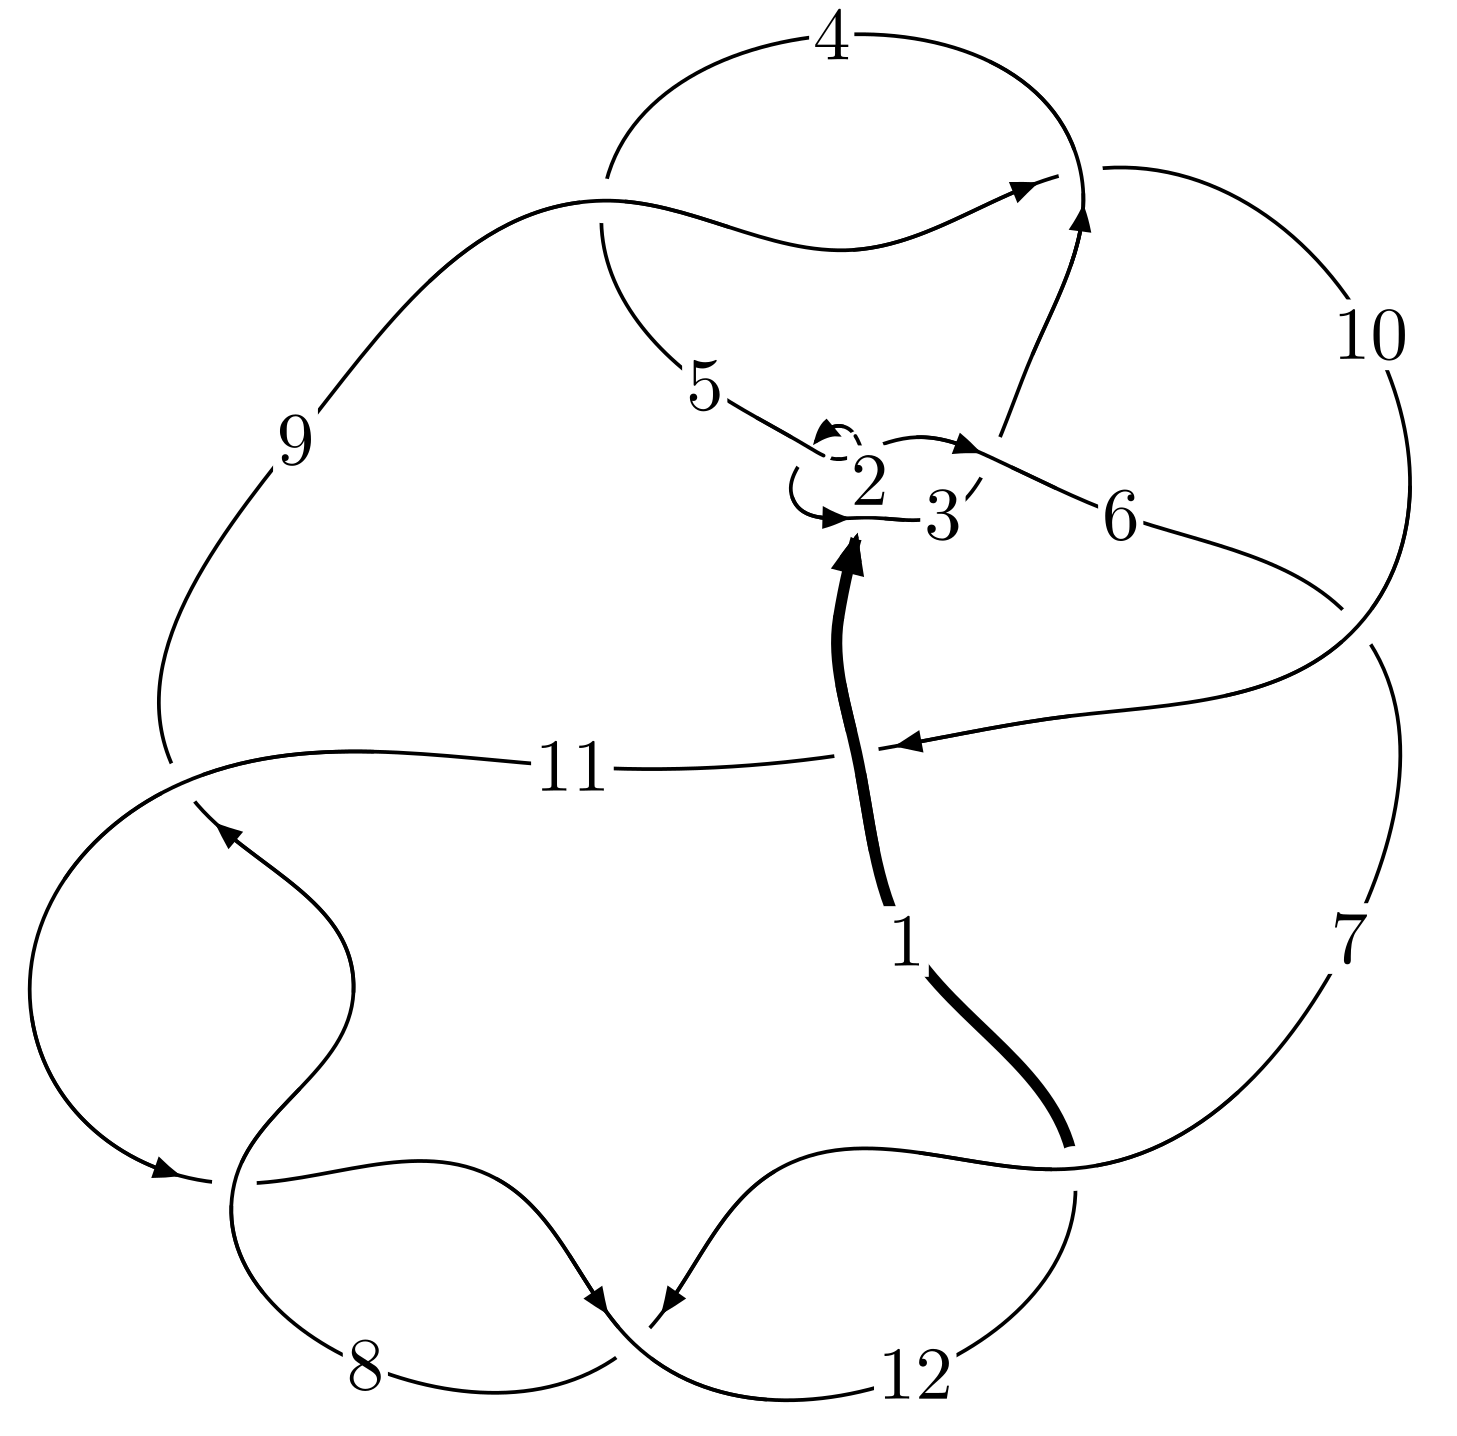
\includegraphics[width=112pt]{../../../GIT/diagram.site/Diagrams/png/823_12a_0022.png}\\
\ \ \ A knot diagram\footnotemark}&
\allowdisplaybreaks
\textbf{Linearized knot diagam} \\
\cline{2-2}
 &
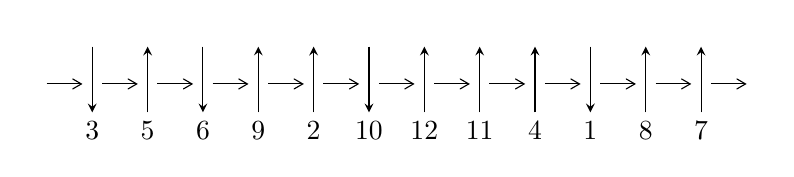
\begin{tikzpicture}[x=20pt, y=17pt]
	% nodes
	\node (C0) at (0, 0) {};
	\node (C1) at (1, 0) {};
	\node (C1U) at (1, +1) {};
	\node (C1D) at (1, -1) {3};

	\node (C2) at (2, 0) {};
	\node (C2U) at (2, +1) {};
	\node (C2D) at (2, -1) {5};

	\node (C3) at (3, 0) {};
	\node (C3U) at (3, +1) {};
	\node (C3D) at (3, -1) {6};

	\node (C4) at (4, 0) {};
	\node (C4U) at (4, +1) {};
	\node (C4D) at (4, -1) {9};

	\node (C5) at (5, 0) {};
	\node (C5U) at (5, +1) {};
	\node (C5D) at (5, -1) {2};

	\node (C6) at (6, 0) {};
	\node (C6U) at (6, +1) {};
	\node (C6D) at (6, -1) {10};

	\node (C7) at (7, 0) {};
	\node (C7U) at (7, +1) {};
	\node (C7D) at (7, -1) {12};

	\node (C8) at (8, 0) {};
	\node (C8U) at (8, +1) {};
	\node (C8D) at (8, -1) {11};

	\node (C9) at (9, 0) {};
	\node (C9U) at (9, +1) {};
	\node (C9D) at (9, -1) {4};

	\node (C10) at (10, 0) {};
	\node (C10U) at (10, +1) {};
	\node (C10D) at (10, -1) {1};

	\node (C11) at (11, 0) {};
	\node (C11U) at (11, +1) {};
	\node (C11D) at (11, -1) {8};

	\node (C12) at (12, 0) {};
	\node (C12U) at (12, +1) {};
	\node (C12D) at (12, -1) {7};
	\node (C13) at (13, 0) {};

	% arrows
	\draw[->,>={angle 60}]
	(C0) edge (C1) (C1) edge (C2) (C2) edge (C3) (C3) edge (C4) (C4) edge (C5) (C5) edge (C6) (C6) edge (C7) (C7) edge (C8) (C8) edge (C9) (C9) edge (C10) (C10) edge (C11) (C11) edge (C12) (C12) edge (C13) ;	\draw[->,>=stealth]
	(C1U) edge (C1D) (C2D) edge (C2U) (C3U) edge (C3D) (C4D) edge (C4U) (C5D) edge (C5U) (C6U) edge (C6D) (C7D) edge (C7U) (C8D) edge (C8U) (C9D) edge (C9U) (C10U) edge (C10D) (C11D) edge (C11U) (C12D) edge (C12U) ;
	\end{tikzpicture} \\
\hhline{~~} \\& 
\textbf{Solving Sequence} \\ \cline{2-2} 
 &
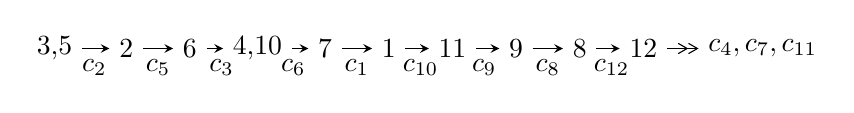
\begin{tikzpicture}[x=23pt, y=7pt]
	% node
	\node (A0) at (-1/8, 0) {3,5};
	\node (A1) at (1, 0) {2};
	\node (A2) at (2, 0) {6};
	\node (A3) at (49/16, 0) {4,10};
	\node (A4) at (33/8, 0) {7};
	\node (A5) at (41/8, 0) {1};
	\node (A6) at (49/8, 0) {11};
	\node (A7) at (57/8, 0) {9};
	\node (A8) at (65/8, 0) {8};
	\node (A9) at (73/8, 0) {12};
	\node (C1) at (1/2, -1) {$c_{2}$};
	\node (C2) at (3/2, -1) {$c_{5}$};
	\node (C3) at (5/2, -1) {$c_{3}$};
	\node (C4) at (29/8, -1) {$c_{6}$};
	\node (C5) at (37/8, -1) {$c_{1}$};
	\node (C6) at (45/8, -1) {$c_{10}$};
	\node (C7) at (53/8, -1) {$c_{9}$};
	\node (C8) at (61/8, -1) {$c_{8}$};
	\node (C9) at (69/8, -1) {$c_{12}$};
	\node (A10) at (11, 0) {$c_{4},c_{7},c_{11}$};

	% edge
	\draw[->,>=stealth]	
	(A0) edge (A1) (A1) edge (A2) (A2) edge (A3) (A3) edge (A4) (A4) edge (A5) (A5) edge (A6) (A6) edge (A7) (A7) edge (A8) (A8) edge (A9) ;
	\draw[->>,>={angle 60}]	
	(A9) edge (A10);
\end{tikzpicture} \\ 

\end{tabular} \\

\footnotetext{
The image of knot diagram is generated by the software ``\textbf{Draw programme}" developed by Andrew Bartholomew(\url{http://www.layer8.co.uk/maths/draw/index.htm\#Running-draw}), where we modified some parts for our purpose(\url{https://github.com/CATsTAILs/LinksPainter}).
}\phantom \\ \newline 
\centering \textbf{Ideals for irreducible components\footnotemark of $X_{\text{par}}$} 
 
\begin{align*}
I^u_{1}&=\langle 
-40 u^{81}+145 u^{80}+\cdots+8 b-29,\;-19 u^{81}+107 u^{80}+\cdots+4 a+41,\;u^{82}-5 u^{81}+\cdots-5 u+1\rangle \\
I^u_{2}&=\langle 
b^4- b^3 u- b^3+b^2 u- u-1,\;a,\;u^2+u+1\rangle \\
\\
\end{align*}
\raggedright * 2 irreducible components of $\dim_{\mathbb{C}}=0$, with total 90 representations.\\
\footnotetext{All coefficients of polynomials are rational numbers. But the coefficients are sometimes approximated in decimal forms when there is not enough margin.}
\newpage
\renewcommand{\arraystretch}{1}
\centering \section*{I. $I^u_{1}= \langle -40 u^{81}+145 u^{80}+\cdots+8 b-29,\;-19 u^{81}+107 u^{80}+\cdots+4 a+41,\;u^{82}-5 u^{81}+\cdots-5 u+1 \rangle$}
\flushleft \textbf{(i) Arc colorings}\\
\begin{tabular}{m{7pt} m{180pt} m{7pt} m{180pt} }
\flushright $a_{3}=$&$\begin{pmatrix}1\\0\end{pmatrix}$ \\
\flushright $a_{5}=$&$\begin{pmatrix}0\\u\end{pmatrix}$ \\
\flushright $a_{2}=$&$\begin{pmatrix}1\\u^2\end{pmatrix}$ \\
\flushright $a_{6}=$&$\begin{pmatrix}u\\u^3+u\end{pmatrix}$ \\
\flushright $a_{4}=$&$\begin{pmatrix}u^4+u^2+1\\u^6+2 u^4+u^2\end{pmatrix}$ \\
\flushright $a_{10}=$&$\begin{pmatrix}4.75000 u^{81}-26.7500 u^{80}+\cdots+42.2500 u-10.2500\\5 u^{81}-\frac{145}{8} u^{80}+\cdots-9 u+\frac{29}{8}\end{pmatrix}$ \\
\flushright $a_{7}=$&$\begin{pmatrix}u^{12}+3 u^{10}+5 u^8-2 u^7+4 u^6-4 u^5+2 u^4-4 u^3+u^2+1\\-\frac{1}{8} u^{81}+\frac{5}{8} u^{80}+\cdots-\frac{5}{8} u+\frac{1}{8}\end{pmatrix}$ \\
\flushright $a_{1}=$&$\begin{pmatrix}u^2+1\\u^2\end{pmatrix}$ \\
\flushright $a_{11}=$&$\begin{pmatrix}6.87500 u^{81}-28.1250 u^{80}+\cdots+13.6250 u-4.12500\\18 u^{81}-74 u^{80}+\cdots+\frac{5}{2} u+\frac{7}{2}\end{pmatrix}$ \\
\flushright $a_{9}=$&$\begin{pmatrix}\frac{23}{4} u^{81}-\frac{103}{4} u^{80}+\cdots+\frac{69}{4} u-\frac{17}{4}\\\frac{61}{4} u^{81}-\frac{509}{8} u^{80}+\cdots+\frac{9}{4} u+\frac{29}{8}\end{pmatrix}$ \\
\flushright $a_{8}=$&$\begin{pmatrix}\frac{11}{2} u^{81}-\frac{105}{4} u^{80}+\cdots+\frac{81}{4} u-\frac{5}{2}\\\frac{13}{2} u^{81}-\frac{251}{8} u^{80}+\cdots+18 u-\frac{25}{8}\end{pmatrix}$ \\
\flushright $a_{12}=$&$\begin{pmatrix}\frac{3}{8} u^{81}-\frac{3}{2} u^{80}+\cdots+\frac{3}{8} u+1\\-\frac{1}{2} u^{81}+\frac{9}{2} u^{80}+\cdots-\frac{43}{4} u+\frac{5}{2}\end{pmatrix}$\\&\end{tabular}
\flushleft \textbf{(ii) Obstruction class $= -1$}\\~\\
\flushleft \textbf{(iii) Cusp Shapes $= \frac{109}{8} u^{81}-\frac{281}{4} u^{80}+\cdots+\frac{271}{8} u+\frac{21}{4}$}\\~\\
\newpage\renewcommand{\arraystretch}{1}
\flushleft \textbf{(iv) u-Polynomials at the component}\newline \\
\begin{tabular}{m{50pt}|m{274pt}}
Crossings & \hspace{64pt}u-Polynomials at each crossing \\
\hline $$\begin{aligned}c_{1}\end{aligned}$$&$\begin{aligned}
&u^{82}+41 u^{81}+\cdots+5 u+1
\end{aligned}$\\
\hline $$\begin{aligned}c_{2},c_{5}\end{aligned}$$&$\begin{aligned}
&u^{82}+5 u^{81}+\cdots+5 u+1
\end{aligned}$\\
\hline $$\begin{aligned}c_{3}\end{aligned}$$&$\begin{aligned}
&u^{82}-5 u^{81}+\cdots+4087 u+1321
\end{aligned}$\\
\hline $$\begin{aligned}c_{4},c_{9}\end{aligned}$$&$\begin{aligned}
&u^{82}+u^{81}+\cdots+128 u+256
\end{aligned}$\\
\hline $$\begin{aligned}c_{6}\end{aligned}$$&$\begin{aligned}
&u^{82}+3 u^{81}+\cdots+81583 u+8329
\end{aligned}$\\
\hline $$\begin{aligned}c_{7},c_{8},c_{11}\\c_{12}\end{aligned}$$&$\begin{aligned}
&u^{82}+3 u^{81}+\cdots+5 u+1
\end{aligned}$\\
\hline $$\begin{aligned}c_{10}\end{aligned}$$&$\begin{aligned}
&u^{82}-23 u^{81}+\cdots-63989 u+3971
\end{aligned}$\\
\hline
\end{tabular}\\~\\
\newpage\renewcommand{\arraystretch}{1}
\flushleft \textbf{(v) Riley Polynomials at the component}\newline \\
\begin{tabular}{m{50pt}|m{274pt}}
Crossings & \hspace{64pt}Riley Polynomials at each crossing \\
\hline $$\begin{aligned}c_{1}\end{aligned}$$&$\begin{aligned}
&y^{82}+5 y^{81}+\cdots+41 y+1
\end{aligned}$\\
\hline $$\begin{aligned}c_{2},c_{5}\end{aligned}$$&$\begin{aligned}
&y^{82}+41 y^{81}+\cdots+5 y+1
\end{aligned}$\\
\hline $$\begin{aligned}c_{3}\end{aligned}$$&$\begin{aligned}
&y^{82}-31 y^{81}+\cdots-31850155 y+1745041
\end{aligned}$\\
\hline $$\begin{aligned}c_{4},c_{9}\end{aligned}$$&$\begin{aligned}
&y^{82}+45 y^{81}+\cdots+1327104 y+65536
\end{aligned}$\\
\hline $$\begin{aligned}c_{6}\end{aligned}$$&$\begin{aligned}
&y^{82}-37 y^{81}+\cdots-2124260175 y+69372241
\end{aligned}$\\
\hline $$\begin{aligned}c_{7},c_{8},c_{11}\\c_{12}\end{aligned}$$&$\begin{aligned}
&y^{82}+95 y^{81}+\cdots+y+1
\end{aligned}$\\
\hline $$\begin{aligned}c_{10}\end{aligned}$$&$\begin{aligned}
&y^{82}-17 y^{81}+\cdots+101206189 y+15768841
\end{aligned}$\\
\hline
\end{tabular}\\~\\
\newpage\flushleft \textbf{(vi) Complex Volumes and Cusp Shapes}
$$\begin{array}{c|c|c}  
\text{Solutions to }I^u_{1}& \I (\text{vol} + \sqrt{-1}CS) & \text{Cusp shape}\\
 \hline 
\begin{aligned}
u &= -0.704314 + 0.732833 I \\
a &= -0.039392 - 0.613136 I \\
b &= -0.383636 + 0.526485 I\end{aligned}
 & -0.38177 - 5.18756 I & \phantom{-0.000000 } 0 \\ \hline\begin{aligned}
u &= -0.704314 - 0.732833 I \\
a &= -0.039392 + 0.613136 I \\
b &= -0.383636 - 0.526485 I\end{aligned}
 & -0.38177 + 5.18756 I & \phantom{-0.000000 } 0 \\ \hline\begin{aligned}
u &= -0.105779 + 0.955141 I \\
a &= -1.38658 - 0.34528 I \\
b &= -0.737097 + 0.693464 I\end{aligned}
 & -8.72790 - 2.31871 I & \phantom{-0.000000 } 0 \\ \hline\begin{aligned}
u &= -0.105779 - 0.955141 I \\
a &= -1.38658 + 0.34528 I \\
b &= -0.737097 - 0.693464 I\end{aligned}
 & -8.72790 + 2.31871 I & \phantom{-0.000000 } 0 \\ \hline\begin{aligned}
u &= -0.741465 + 0.744493 I \\
a &= \phantom{-}0.296277 + 0.595555 I \\
b &= \phantom{-}0.501466 - 0.980876 I\end{aligned}
 & -8.14095 - 7.21306 I & \phantom{-0.000000 } 0 \\ \hline\begin{aligned}
u &= -0.741465 - 0.744493 I \\
a &= \phantom{-}0.296277 - 0.595555 I \\
b &= \phantom{-}0.501466 + 0.980876 I\end{aligned}
 & -8.14095 + 7.21306 I & \phantom{-0.000000 } 0 \\ \hline\begin{aligned}
u &= -0.625049 + 0.701797 I \\
a &= -0.378967 + 0.585059 I \\
b &= \phantom{-}0.198631 + 0.083439 I\end{aligned}
 & \phantom{-}1.02352 - 2.11165 I & \phantom{-0.000000 } 0 \\ \hline\begin{aligned}
u &= -0.625049 - 0.701797 I \\
a &= -0.378967 - 0.585059 I \\
b &= \phantom{-}0.198631 - 0.083439 I\end{aligned}
 & \phantom{-}1.02352 + 2.11165 I & \phantom{-0.000000 } 0 \\ \hline\begin{aligned}
u &= -0.567368 + 0.920415 I \\
a &= -0.378006 + 0.357257 I \\
b &= -0.244076 + 0.661524 I\end{aligned}
 & \phantom{-}0.39375 - 2.56563 I & \phantom{-0.000000 } 0 \\ \hline\begin{aligned}
u &= -0.567368 - 0.920415 I \\
a &= -0.378006 - 0.357257 I \\
b &= -0.244076 - 0.661524 I\end{aligned}
 & \phantom{-}0.39375 + 2.56563 I & \phantom{-0.000000 } 0\\
 \hline 
 \end{array}$$\newpage$$\begin{array}{c|c|c}  
\text{Solutions to }I^u_{1}& \I (\text{vol} + \sqrt{-1}CS) & \text{Cusp shape}\\
 \hline 
\begin{aligned}
u &= -0.659941 + 0.872179 I \\
a &= \phantom{-}0.277339 - 0.046151 I \\
b &= \phantom{-}0.879179 + 0.019524 I\end{aligned}
 & -0.794028 - 0.020453 I & \phantom{-0.000000 } 0 \\ \hline\begin{aligned}
u &= -0.659941 - 0.872179 I \\
a &= \phantom{-}0.277339 + 0.046151 I \\
b &= \phantom{-}0.879179 - 0.019524 I\end{aligned}
 & -0.794028 + 0.020453 I & \phantom{-0.000000 } 0 \\ \hline\begin{aligned}
u &= \phantom{-}0.854489 + 0.292104 I \\
a &= -2.34167 + 0.05715 I \\
b &= -2.00466 - 0.97235 I\end{aligned}
 & -10.7779 - 10.0786 I & \phantom{-0.000000 } 0 \\ \hline\begin{aligned}
u &= \phantom{-}0.854489 - 0.292104 I \\
a &= -2.34167 - 0.05715 I \\
b &= -2.00466 + 0.97235 I\end{aligned}
 & -10.7779 + 10.0786 I & \phantom{-0.000000 } 0 \\ \hline\begin{aligned}
u &= \phantom{-}0.410592 + 1.038090 I \\
a &= -0.128468 - 0.117863 I \\
b &= -1.282850 + 0.198070 I\end{aligned}
 & -7.98722 - 0.83968 I & \phantom{-0.000000 } 0 \\ \hline\begin{aligned}
u &= \phantom{-}0.410592 - 1.038090 I \\
a &= -0.128468 + 0.117863 I \\
b &= -1.282850 - 0.198070 I\end{aligned}
 & -7.98722 + 0.83968 I & \phantom{-0.000000 } 0 \\ \hline\begin{aligned}
u &= \phantom{-}0.829105 + 0.286958 I \\
a &= \phantom{-}2.10320 - 0.00102 I \\
b &= \phantom{-}1.63515 + 0.78199 I\end{aligned}
 & -2.85556 - 7.68645 I & \phantom{-0.000000 } 0 \\ \hline\begin{aligned}
u &= \phantom{-}0.829105 - 0.286958 I \\
a &= \phantom{-}2.10320 + 0.00102 I \\
b &= \phantom{-}1.63515 - 0.78199 I\end{aligned}
 & -2.85556 + 7.68645 I & \phantom{-0.000000 } 0 \\ \hline\begin{aligned}
u &= -0.701766 + 0.880022 I \\
a &= -0.179014 - 0.153824 I \\
b &= -1.302540 - 0.384385 I\end{aligned}
 & -8.54157 + 1.77332 I & \phantom{-0.000000 } 0 \\ \hline\begin{aligned}
u &= -0.701766 - 0.880022 I \\
a &= -0.179014 + 0.153824 I \\
b &= -1.302540 + 0.384385 I\end{aligned}
 & -8.54157 - 1.77332 I & \phantom{-0.000000 } 0\\
 \hline 
 \end{array}$$\newpage$$\begin{array}{c|c|c}  
\text{Solutions to }I^u_{1}& \I (\text{vol} + \sqrt{-1}CS) & \text{Cusp shape}\\
 \hline 
\begin{aligned}
u &= \phantom{-}0.835427 + 0.163941 I \\
a &= -1.43377 + 0.88175 I \\
b &= -1.58005 + 0.86107 I\end{aligned}
 & -12.74480 + 0.10746 I & -3.09571 + 0. I\phantom{ +0.000000I} \\ \hline\begin{aligned}
u &= \phantom{-}0.835427 - 0.163941 I \\
a &= -1.43377 - 0.88175 I \\
b &= -1.58005 - 0.86107 I\end{aligned}
 & -12.74480 - 0.10746 I & -3.09571 + 0. I\phantom{ +0.000000I} \\ \hline\begin{aligned}
u &= -0.228543 + 0.813377 I \\
a &= \phantom{-}1.064610 + 0.363456 I \\
b &= \phantom{-}0.610969 - 0.498748 I\end{aligned}
 & -1.37873 - 1.65649 I & -3.71571 + 4.84793 I \\ \hline\begin{aligned}
u &= -0.228543 - 0.813377 I \\
a &= \phantom{-}1.064610 - 0.363456 I \\
b &= \phantom{-}0.610969 + 0.498748 I\end{aligned}
 & -1.37873 + 1.65649 I & -3.71571 - 4.84793 I \\ \hline\begin{aligned}
u &= \phantom{-}0.447742 + 1.064870 I \\
a &= \phantom{-}0.026648 + 0.300164 I \\
b &= \phantom{-}0.936468 + 0.133542 I\end{aligned}
 & -1.27806 + 1.55480 I & \phantom{-0.000000 } 0 \\ \hline\begin{aligned}
u &= \phantom{-}0.447742 - 1.064870 I \\
a &= \phantom{-}0.026648 - 0.300164 I \\
b &= \phantom{-}0.936468 - 0.133542 I\end{aligned}
 & -1.27806 - 1.55480 I & \phantom{-0.000000 } 0 \\ \hline\begin{aligned}
u &= -0.401903 + 1.086010 I \\
a &= -0.50943 - 1.80938 I \\
b &= -1.94745 - 0.21375 I\end{aligned}
 & -3.10543 - 0.73820 I & \phantom{-0.000000 } 0 \\ \hline\begin{aligned}
u &= -0.401903 - 1.086010 I \\
a &= -0.50943 + 1.80938 I \\
b &= -1.94745 + 0.21375 I\end{aligned}
 & -3.10543 + 0.73820 I & \phantom{-0.000000 } 0 \\ \hline\begin{aligned}
u &= \phantom{-}0.792544 + 0.272348 I \\
a &= -1.77905 - 0.02879 I \\
b &= -1.224390 - 0.466760 I\end{aligned}
 & -1.18892 - 3.99153 I & \phantom{-}4.00000 + 2.29977 I \\ \hline\begin{aligned}
u &= \phantom{-}0.792544 - 0.272348 I \\
a &= -1.77905 + 0.02879 I \\
b &= -1.224390 + 0.466760 I\end{aligned}
 & -1.18892 + 3.99153 I & \phantom{-}4.00000 - 2.29977 I\\
 \hline 
 \end{array}$$\newpage$$\begin{array}{c|c|c}  
\text{Solutions to }I^u_{1}& \I (\text{vol} + \sqrt{-1}CS) & \text{Cusp shape}\\
 \hline 
\begin{aligned}
u &= -0.646960 + 0.529804 I \\
a &= \phantom{-}1.00756 - 1.18930 I \\
b &= -0.436228 - 1.048150 I\end{aligned}
 & -4.34258 - 1.45718 I & \phantom{-}4.00000 + 3.03293 I \\ \hline\begin{aligned}
u &= -0.646960 - 0.529804 I \\
a &= \phantom{-}1.00756 + 1.18930 I \\
b &= -0.436228 + 1.048150 I\end{aligned}
 & -4.34258 + 1.45718 I & \phantom{-}4.00000 - 3.03293 I \\ \hline\begin{aligned}
u &= -0.585550 + 1.006890 I \\
a &= \phantom{-}0.847118 - 0.654790 I \\
b &= \phantom{-}0.14547 - 1.74184 I\end{aligned}
 & -5.72135 - 3.35594 I & \phantom{-0.000000 } 0 \\ \hline\begin{aligned}
u &= -0.585550 - 1.006890 I \\
a &= \phantom{-}0.847118 + 0.654790 I \\
b &= \phantom{-}0.14547 + 1.74184 I\end{aligned}
 & -5.72135 + 3.35594 I & \phantom{-0.000000 } 0 \\ \hline\begin{aligned}
u &= -0.473787 + 1.064880 I \\
a &= -0.18710 + 1.59396 I \\
b &= \phantom{-}1.60049 + 1.10893 I\end{aligned}
 & -0.74392 - 3.35669 I & \phantom{-0.000000 } 0 \\ \hline\begin{aligned}
u &= -0.473787 - 1.064880 I \\
a &= -0.18710 - 1.59396 I \\
b &= \phantom{-}1.60049 - 1.10893 I\end{aligned}
 & -0.74392 + 3.35669 I & \phantom{-0.000000 } 0 \\ \hline\begin{aligned}
u &= \phantom{-}0.480590 + 1.080350 I \\
a &= -0.007942 - 0.520219 I \\
b &= -0.542127 - 0.479128 I\end{aligned}
 & -0.99744 + 5.35792 I & \phantom{-0.000000 } 0 \\ \hline\begin{aligned}
u &= \phantom{-}0.480590 - 1.080350 I \\
a &= -0.007942 + 0.520219 I \\
b &= -0.542127 + 0.479128 I\end{aligned}
 & -0.99744 - 5.35792 I & \phantom{-0.000000 } 0 \\ \hline\begin{aligned}
u &= \phantom{-}0.786259 + 0.197156 I \\
a &= \phantom{-}1.39080 - 0.38724 I \\
b &= \phantom{-}1.192400 - 0.326068 I\end{aligned}
 & -4.31599 - 1.20763 I & -1.64666 - 0.57039 I \\ \hline\begin{aligned}
u &= \phantom{-}0.786259 - 0.197156 I \\
a &= \phantom{-}1.39080 + 0.38724 I \\
b &= \phantom{-}1.192400 + 0.326068 I\end{aligned}
 & -4.31599 + 1.20763 I & -1.64666 + 0.57039 I\\
 \hline 
 \end{array}$$\newpage$$\begin{array}{c|c|c}  
\text{Solutions to }I^u_{1}& \I (\text{vol} + \sqrt{-1}CS) & \text{Cusp shape}\\
 \hline 
\begin{aligned}
u &= -0.387160 + 1.125240 I \\
a &= \phantom{-}0.74985 + 2.17217 I \\
b &= \phantom{-}2.37416 - 0.11109 I\end{aligned}
 & -11.12530 + 0.93298 I & \phantom{-0.000000 } 0 \\ \hline\begin{aligned}
u &= -0.387160 - 1.125240 I \\
a &= \phantom{-}0.74985 - 2.17217 I \\
b &= \phantom{-}2.37416 + 0.11109 I\end{aligned}
 & -11.12530 - 0.93298 I & \phantom{-0.000000 } 0 \\ \hline\begin{aligned}
u &= \phantom{-}0.520504 + 1.092360 I \\
a &= \phantom{-}0.095680 + 0.832445 I \\
b &= -0.021566 + 1.043640 I\end{aligned}
 & -7.02432 + 7.67620 I & \phantom{-0.000000 } 0 \\ \hline\begin{aligned}
u &= \phantom{-}0.520504 - 1.092360 I \\
a &= \phantom{-}0.095680 - 0.832445 I \\
b &= -0.021566 - 1.043640 I\end{aligned}
 & -7.02432 - 7.67620 I & \phantom{-0.000000 } 0 \\ \hline\begin{aligned}
u &= -0.489951 + 1.107000 I \\
a &= \phantom{-}0.44869 - 2.01555 I \\
b &= -2.19473 - 1.55021 I\end{aligned}
 & -2.46183 - 6.60369 I & \phantom{-0.000000 } 0 \\ \hline\begin{aligned}
u &= -0.489951 - 1.107000 I \\
a &= \phantom{-}0.44869 + 2.01555 I \\
b &= -2.19473 + 1.55021 I\end{aligned}
 & -2.46183 + 6.60369 I & \phantom{-0.000000 } 0 \\ \hline\begin{aligned}
u &= \phantom{-}0.278575 + 1.179870 I \\
a &= -0.079195 - 1.106280 I \\
b &= \phantom{-}1.35992 - 0.65097 I\end{aligned}
 & -5.69304 - 0.73230 I & \phantom{-0.000000 } 0 \\ \hline\begin{aligned}
u &= \phantom{-}0.278575 - 1.179870 I \\
a &= -0.079195 + 1.106280 I \\
b &= \phantom{-}1.35992 + 0.65097 I\end{aligned}
 & -5.69304 + 0.73230 I & \phantom{-0.000000 } 0 \\ \hline\begin{aligned}
u &= \phantom{-}0.252443 + 1.203480 I \\
a &= -0.05183 + 1.44329 I \\
b &= -1.47746 + 0.48712 I\end{aligned}
 & -7.63888 - 4.38566 I & \phantom{-0.000000 } 0 \\ \hline\begin{aligned}
u &= \phantom{-}0.252443 - 1.203480 I \\
a &= -0.05183 - 1.44329 I \\
b &= -1.47746 - 0.48712 I\end{aligned}
 & -7.63888 + 4.38566 I & \phantom{-0.000000 } 0\\
 \hline 
 \end{array}$$\newpage$$\begin{array}{c|c|c}  
\text{Solutions to }I^u_{1}& \I (\text{vol} + \sqrt{-1}CS) & \text{Cusp shape}\\
 \hline 
\begin{aligned}
u &= -0.494792 + 1.131070 I \\
a &= -0.56672 + 2.31046 I \\
b &= \phantom{-}2.65647 + 1.74358 I\end{aligned}
 & -10.36760 - 8.71428 I & \phantom{-0.000000 } 0 \\ \hline\begin{aligned}
u &= -0.494792 - 1.131070 I \\
a &= -0.56672 - 2.31046 I \\
b &= \phantom{-}2.65647 - 1.74358 I\end{aligned}
 & -10.36760 + 8.71428 I & \phantom{-0.000000 } 0 \\ \hline\begin{aligned}
u &= \phantom{-}0.322106 + 1.195250 I \\
a &= \phantom{-}0.527321 + 0.957086 I \\
b &= -1.34997 + 0.92937 I\end{aligned}
 & -8.57034 + 2.40449 I & \phantom{-0.000000 } 0 \\ \hline\begin{aligned}
u &= \phantom{-}0.322106 - 1.195250 I \\
a &= \phantom{-}0.527321 - 0.957086 I \\
b &= -1.34997 - 0.92937 I\end{aligned}
 & -8.57034 - 2.40449 I & \phantom{-0.000000 } 0 \\ \hline\begin{aligned}
u &= \phantom{-}0.241449 + 1.225680 I \\
a &= \phantom{-}0.08124 - 1.72667 I \\
b &= \phantom{-}1.60146 - 0.35341 I\end{aligned}
 & -15.7352 - 6.6947 I & \phantom{-0.000000 } 0 \\ \hline\begin{aligned}
u &= \phantom{-}0.241449 - 1.225680 I \\
a &= \phantom{-}0.08124 + 1.72667 I \\
b &= \phantom{-}1.60146 + 0.35341 I\end{aligned}
 & -15.7352 + 6.6947 I & \phantom{-0.000000 } 0 \\ \hline\begin{aligned}
u &= \phantom{-}0.633300 + 0.364129 I \\
a &= \phantom{-}1.146130 + 0.757063 I \\
b &= -0.206752 + 0.243475 I\end{aligned}
 & -4.89815 - 3.14508 I & \phantom{-}2.29655 + 3.69057 I \\ \hline\begin{aligned}
u &= \phantom{-}0.633300 - 0.364129 I \\
a &= \phantom{-}1.146130 - 0.757063 I \\
b &= -0.206752 - 0.243475 I\end{aligned}
 & -4.89815 + 3.14508 I & \phantom{-}2.29655 - 3.69057 I \\ \hline\begin{aligned}
u &= \phantom{-}0.338253 + 1.225240 I \\
a &= -0.917777 - 1.065290 I \\
b &= \phantom{-}1.49348 - 1.21156 I\end{aligned}
 & -17.0811 + 4.0269 I & \phantom{-0.000000 } 0 \\ \hline\begin{aligned}
u &= \phantom{-}0.338253 - 1.225240 I \\
a &= -0.917777 + 1.065290 I \\
b &= \phantom{-}1.49348 + 1.21156 I\end{aligned}
 & -17.0811 - 4.0269 I & \phantom{-0.000000 } 0\\
 \hline 
 \end{array}$$\newpage$$\begin{array}{c|c|c}  
\text{Solutions to }I^u_{1}& \I (\text{vol} + \sqrt{-1}CS) & \text{Cusp shape}\\
 \hline 
\begin{aligned}
u &= \phantom{-}0.529169 + 1.165730 I \\
a &= -0.55607 + 1.33364 I \\
b &= -1.49781 + 0.01915 I\end{aligned}
 & -7.15078 + 6.07252 I & \phantom{-0.000000 } 0 \\ \hline\begin{aligned}
u &= \phantom{-}0.529169 - 1.165730 I \\
a &= -0.55607 - 1.33364 I \\
b &= -1.49781 - 0.01915 I\end{aligned}
 & -7.15078 - 6.07252 I & \phantom{-0.000000 } 0 \\ \hline\begin{aligned}
u &= \phantom{-}0.556937 + 1.154960 I \\
a &= \phantom{-}0.23026 - 1.59190 I \\
b &= \phantom{-}1.89941 - 0.80869 I\end{aligned}
 & -3.79190 + 9.02671 I & \phantom{-0.000000 } 0 \\ \hline\begin{aligned}
u &= \phantom{-}0.556937 - 1.154960 I \\
a &= \phantom{-}0.23026 + 1.59190 I \\
b &= \phantom{-}1.89941 + 0.80869 I\end{aligned}
 & -3.79190 - 9.02671 I & \phantom{-0.000000 } 0 \\ \hline\begin{aligned}
u &= \phantom{-}0.571315 + 1.163160 I \\
a &= -0.20043 + 1.83707 I \\
b &= -2.42638 + 0.96617 I\end{aligned}
 & -5.46594 + 12.87520 I & \phantom{-0.000000 } 0 \\ \hline\begin{aligned}
u &= \phantom{-}0.571315 - 1.163160 I \\
a &= -0.20043 - 1.83707 I \\
b &= -2.42638 - 0.96617 I\end{aligned}
 & -5.46594 - 12.87520 I & \phantom{-0.000000 } 0 \\ \hline\begin{aligned}
u &= \phantom{-}0.358574 + 0.605548 I \\
a &= -0.725871 - 0.684487 I \\
b &= \phantom{-}0.181111 + 1.173260 I\end{aligned}
 & -6.57846 + 4.17153 I & -0.218037 + 0.553666 I \\ \hline\begin{aligned}
u &= \phantom{-}0.358574 - 0.605548 I \\
a &= -0.725871 + 0.684487 I \\
b &= \phantom{-}0.181111 - 1.173260 I\end{aligned}
 & -6.57846 - 4.17153 I & -0.218037 - 0.553666 I \\ \hline\begin{aligned}
u &= \phantom{-}0.522003 + 1.192470 I \\
a &= \phantom{-}0.95599 - 1.38115 I \\
b &= \phantom{-}1.72988 + 0.74459 I\end{aligned}
 & -15.8138 + 4.8468 I & \phantom{-0.000000 } 0 \\ \hline\begin{aligned}
u &= \phantom{-}0.522003 - 1.192470 I \\
a &= \phantom{-}0.95599 + 1.38115 I \\
b &= \phantom{-}1.72988 - 0.74459 I\end{aligned}
 & -15.8138 - 4.8468 I & \phantom{-0.000000 } 0\\
 \hline 
 \end{array}$$\newpage$$\begin{array}{c|c|c}  
\text{Solutions to }I^u_{1}& \I (\text{vol} + \sqrt{-1}CS) & \text{Cusp shape}\\
 \hline 
\begin{aligned}
u &= \phantom{-}0.580577 + 1.170980 I \\
a &= \phantom{-}0.20698 - 2.03262 I \\
b &= \phantom{-}2.86387 - 1.01322 I\end{aligned}
 & -13.4120 + 15.3715 I & \phantom{-0.000000 } 0 \\ \hline\begin{aligned}
u &= \phantom{-}0.580577 - 1.170980 I \\
a &= \phantom{-}0.20698 + 2.03262 I \\
b &= \phantom{-}2.86387 + 1.01322 I\end{aligned}
 & -13.4120 - 15.3715 I & \phantom{-0.000000 } 0 \\ \hline\begin{aligned}
u &= -0.633105 + 0.172755 I \\
a &= -2.82368 + 0.73281 I \\
b &= -1.72041 + 1.20662 I\end{aligned}
 & -7.70310 + 4.34280 I & \phantom{-}1.05723 - 2.52323 I \\ \hline\begin{aligned}
u &= -0.633105 - 0.172755 I \\
a &= -2.82368 - 0.73281 I \\
b &= -1.72041 - 1.20662 I\end{aligned}
 & -7.70310 - 4.34280 I & \phantom{-}1.05723 + 2.52323 I \\ \hline\begin{aligned}
u &= -0.469905 + 0.400587 I \\
a &= -1.70527 + 0.49698 I \\
b &= -0.460855 + 0.893450 I\end{aligned}
 & \phantom{-}1.183240 - 0.630202 I & \phantom{-}8.42558 + 2.80238 I \\ \hline\begin{aligned}
u &= -0.469905 - 0.400587 I \\
a &= -1.70527 - 0.49698 I \\
b &= -0.460855 - 0.893450 I\end{aligned}
 & \phantom{-}1.183240 + 0.630202 I & \phantom{-}8.42558 - 2.80238 I \\ \hline\begin{aligned}
u &= \phantom{-}0.353527 + 0.489455 I \\
a &= \phantom{-}0.831523 + 0.783639 I \\
b &= -0.196486 - 0.779621 I\end{aligned}
 & \phantom{-}0.57076 + 2.04372 I & \phantom{-}3.58253 - 2.28115 I \\ \hline\begin{aligned}
u &= \phantom{-}0.353527 - 0.489455 I \\
a &= \phantom{-}0.831523 - 0.783639 I \\
b &= -0.196486 + 0.779621 I\end{aligned}
 & \phantom{-}0.57076 - 2.04372 I & \phantom{-}3.58253 + 2.28115 I \\ \hline\begin{aligned}
u &= -0.550775 + 0.221389 I \\
a &= \phantom{-}2.42931 - 0.59762 I \\
b &= \phantom{-}1.16401 - 1.01324 I\end{aligned}
 & -0.02868 + 2.38938 I & \phantom{-}3.67522 - 4.58945 I \\ \hline\begin{aligned}
u &= -0.550775 - 0.221389 I \\
a &= \phantom{-}2.42931 + 0.59762 I \\
b &= \phantom{-}1.16401 + 1.01324 I\end{aligned}
 & -0.02868 - 2.38938 I & \phantom{-}3.67522 + 4.58945 I\\
 \hline 
 \end{array}$$\newpage$$\begin{array}{c|c|c}  
\text{Solutions to }I^u_{1}& \I (\text{vol} + \sqrt{-1}CS) & \text{Cusp shape}\\
 \hline 
\begin{aligned}
u &= \phantom{-}0.472632 + 0.351594 I \\
a &= -0.840285 - 0.800430 I \\
b &= \phantom{-}0.213524 + 0.348569 I\end{aligned}
 & \phantom{-}1.10262 - 1.31646 I & \phantom{-}6.13864 + 5.00378 I \\ \hline\begin{aligned}
u &= \phantom{-}0.472632 - 0.351594 I \\
a &= -0.840285 + 0.800430 I \\
b &= \phantom{-}0.213524 - 0.348569 I\end{aligned}
 & \phantom{-}1.10262 + 1.31646 I & \phantom{-}6.13864 - 5.00378 I\\
 \hline 
 \end{array}$$\newpage\newpage\renewcommand{\arraystretch}{1}
\centering \section*{II. $I^u_{2}= \langle b^4- b^3 u- b^3+b^2 u- u-1,\;a,\;u^2+u+1 \rangle$}
\flushleft \textbf{(i) Arc colorings}\\
\begin{tabular}{m{7pt} m{180pt} m{7pt} m{180pt} }
\flushright $a_{3}=$&$\begin{pmatrix}1\\0\end{pmatrix}$ \\
\flushright $a_{5}=$&$\begin{pmatrix}0\\u\end{pmatrix}$ \\
\flushright $a_{2}=$&$\begin{pmatrix}1\\- u-1\end{pmatrix}$ \\
\flushright $a_{6}=$&$\begin{pmatrix}u\\u+1\end{pmatrix}$ \\
\flushright $a_{4}=$&$\begin{pmatrix}0\\u\end{pmatrix}$ \\
\flushright $a_{10}=$&$\begin{pmatrix}0\\b\end{pmatrix}$ \\
\flushright $a_{7}=$&$\begin{pmatrix}u\\b^2 u+u+1\end{pmatrix}$ \\
\flushright $a_{1}=$&$\begin{pmatrix}- u\\- u-1\end{pmatrix}$ \\
\flushright $a_{11}=$&$\begin{pmatrix}b u+b\\2 b\end{pmatrix}$ \\
\flushright $a_{9}=$&$\begin{pmatrix}0\\b\end{pmatrix}$ \\
\flushright $a_{8}=$&$\begin{pmatrix}- b^3 u\\-2 b^3 u-2 b^3+b\end{pmatrix}$ \\
\flushright $a_{12}=$&$\begin{pmatrix}- b^2- u\\- b^3 u- b^3+2 b^2 u-2 u-2\end{pmatrix}$\\&\end{tabular}
\flushleft \textbf{(ii) Obstruction class $= 1$}\\~\\
\flushleft \textbf{(iii) Cusp Shapes $= -5 b^2 u-3 b^2+3 b u- b+5 u+6$}\\~\\
\newpage\renewcommand{\arraystretch}{1}
\flushleft \textbf{(iv) u-Polynomials at the component}\newline \\
\begin{tabular}{m{50pt}|m{274pt}}
Crossings & \hspace{64pt}u-Polynomials at each crossing \\
\hline $$\begin{aligned}c_{1},c_{3},c_{5}\end{aligned}$$&$\begin{aligned}
&(u^2- u+1)^4
\end{aligned}$\\
\hline $$\begin{aligned}c_{2}\end{aligned}$$&$\begin{aligned}
&(u^2+u+1)^4
\end{aligned}$\\
\hline $$\begin{aligned}c_{4},c_{9}\end{aligned}$$&$\begin{aligned}
&u^8
\end{aligned}$\\
\hline $$\begin{aligned}c_{6},c_{10}\end{aligned}$$&$\begin{aligned}
&(u^4+u^3+u^2+1)^2
\end{aligned}$\\
\hline $$\begin{aligned}c_{7},c_{8}\end{aligned}$$&$\begin{aligned}
&(u^4+u^3+3 u^2+2 u+1)^2
\end{aligned}$\\
\hline $$\begin{aligned}c_{11},c_{12}\end{aligned}$$&$\begin{aligned}
&(u^4- u^3+3 u^2-2 u+1)^2
\end{aligned}$\\
\hline
\end{tabular}\\~\\
\newpage\renewcommand{\arraystretch}{1}
\flushleft \textbf{(v) Riley Polynomials at the component}\newline \\
\begin{tabular}{m{50pt}|m{274pt}}
Crossings & \hspace{64pt}Riley Polynomials at each crossing \\
\hline $$\begin{aligned}c_{1},c_{2},c_{3}\\c_{5}\end{aligned}$$&$\begin{aligned}
&(y^2+y+1)^4
\end{aligned}$\\
\hline $$\begin{aligned}c_{4},c_{9}\end{aligned}$$&$\begin{aligned}
&y^8
\end{aligned}$\\
\hline $$\begin{aligned}c_{6},c_{10}\end{aligned}$$&$\begin{aligned}
&(y^4+y^3+3 y^2+2 y+1)^2
\end{aligned}$\\
\hline $$\begin{aligned}c_{7},c_{8},c_{11}\\c_{12}\end{aligned}$$&$\begin{aligned}
&(y^4+5 y^3+7 y^2+2 y+1)^2
\end{aligned}$\\
\hline
\end{tabular}\\~\\
\newpage\flushleft \textbf{(vi) Complex Volumes and Cusp Shapes}
$$\begin{array}{c|c|c}  
\text{Solutions to }I^u_{2}& \I (\text{vol} + \sqrt{-1}CS) & \text{Cusp shape}\\
 \hline 
\begin{aligned}
u &= -0.500000 + 0.866025 I \\
a &= \phantom{-0.000000 } 0 \\
b &= \phantom{-}0.447930 - 0.664845 I\end{aligned}
 & \phantom{-}0.21101 - 3.44499 I & \phantom{-}1.64912 + 8.49900 I \\ \hline\begin{aligned}
u &= -0.500000 + 0.866025 I \\
a &= \phantom{-0.000000 } 0 \\
b &= -0.799738 + 0.055496 I\end{aligned}
 & \phantom{-}0.211005 - 0.614778 I & \phantom{-}4.65255 - 0.59814 I \\ \hline\begin{aligned}
u &= -0.500000 + 0.866025 I \\
a &= \phantom{-0.000000 } 0 \\
b &= -0.363298 + 1.193330 I\end{aligned}
 & -6.79074 - 5.19385 I & -1.80063 + 6.43123 I \\ \hline\begin{aligned}
u &= -0.500000 + 0.866025 I \\
a &= \phantom{-0.000000 } 0 \\
b &= \phantom{-}1.215110 + 0.282041 I\end{aligned}
 & -6.79074 + 1.13408 I & \phantom{-}1.99896 + 0.39034 I \\ \hline\begin{aligned}
u &= -0.500000 - 0.866025 I \\
a &= \phantom{-0.000000 } 0 \\
b &= \phantom{-}0.447930 + 0.664845 I\end{aligned}
 & \phantom{-}0.21101 + 3.44499 I & \phantom{-}1.64912 - 8.49900 I \\ \hline\begin{aligned}
u &= -0.500000 - 0.866025 I \\
a &= \phantom{-0.000000 } 0 \\
b &= -0.799738 - 0.055496 I\end{aligned}
 & \phantom{-}0.211005 + 0.614778 I & \phantom{-}4.65255 + 0.59814 I \\ \hline\begin{aligned}
u &= -0.500000 - 0.866025 I \\
a &= \phantom{-0.000000 } 0 \\
b &= -0.363298 - 1.193330 I\end{aligned}
 & -6.79074 + 5.19385 I & -1.80063 - 6.43123 I \\ \hline\begin{aligned}
u &= -0.500000 - 0.866025 I \\
a &= \phantom{-0.000000 } 0 \\
b &= \phantom{-}1.215110 - 0.282041 I\end{aligned}
 & -6.79074 - 1.13408 I & \phantom{-}1.99896 - 0.39034 I\\
 \hline 
 \end{array}$$\newpage
\newpage\renewcommand{\arraystretch}{1}
\centering \section*{ III. u-Polynomials}
\begin{tabular}{m{50pt}|m{274pt}}
Crossings & \hspace{64pt}u-Polynomials at each crossing \\
\hline $$\begin{aligned}c_{1}\end{aligned}$$&$\begin{aligned}
&((u^2- u+1)^4)(u^{82}+41 u^{81}+\cdots+5 u+1)
\end{aligned}$\\
\hline $$\begin{aligned}c_{2}\end{aligned}$$&$\begin{aligned}
&((u^2+u+1)^4)(u^{82}+5 u^{81}+\cdots+5 u+1)
\end{aligned}$\\
\hline $$\begin{aligned}c_{3}\end{aligned}$$&$\begin{aligned}
&((u^2- u+1)^4)(u^{82}-5 u^{81}+\cdots+4087 u+1321)
\end{aligned}$\\
\hline $$\begin{aligned}c_{4},c_{9}\end{aligned}$$&$\begin{aligned}
&u^8(u^{82}+u^{81}+\cdots+128 u+256)
\end{aligned}$\\
\hline $$\begin{aligned}c_{5}\end{aligned}$$&$\begin{aligned}
&((u^2- u+1)^4)(u^{82}+5 u^{81}+\cdots+5 u+1)
\end{aligned}$\\
\hline $$\begin{aligned}c_{6}\end{aligned}$$&$\begin{aligned}
&((u^4+u^3+u^2+1)^2)(u^{82}+3 u^{81}+\cdots+81583 u+8329)
\end{aligned}$\\
\hline $$\begin{aligned}c_{7},c_{8}\end{aligned}$$&$\begin{aligned}
&((u^4+u^3+3 u^2+2 u+1)^2)(u^{82}+3 u^{81}+\cdots+5 u+1)
\end{aligned}$\\
\hline $$\begin{aligned}c_{10}\end{aligned}$$&$\begin{aligned}
&((u^4+u^3+u^2+1)^2)(u^{82}-23 u^{81}+\cdots-63989 u+3971)
\end{aligned}$\\
\hline $$\begin{aligned}c_{11},c_{12}\end{aligned}$$&$\begin{aligned}
&((u^4- u^3+3 u^2-2 u+1)^2)(u^{82}+3 u^{81}+\cdots+5 u+1)
\end{aligned}$\\
\hline
\end{tabular}\newpage\renewcommand{\arraystretch}{1}
\centering \section*{ IV. Riley Polynomials}
\begin{tabular}{m{50pt}|m{274pt}}
Crossings & \hspace{64pt}Riley Polynomials at each crossing \\
\hline $$\begin{aligned}c_{1}\end{aligned}$$&$\begin{aligned}
&((y^2+y+1)^4)(y^{82}+5 y^{81}+\cdots+41 y+1)
\end{aligned}$\\
\hline $$\begin{aligned}c_{2},c_{5}\end{aligned}$$&$\begin{aligned}
&((y^2+y+1)^4)(y^{82}+41 y^{81}+\cdots+5 y+1)
\end{aligned}$\\
\hline $$\begin{aligned}c_{3}\end{aligned}$$&$\begin{aligned}
&((y^2+y+1)^4)(y^{82}-31 y^{81}+\cdots-3.18502\times10^{7} y+1745041)
\end{aligned}$\\
\hline $$\begin{aligned}c_{4},c_{9}\end{aligned}$$&$\begin{aligned}
&y^8(y^{82}+45 y^{81}+\cdots+1327104 y+65536)
\end{aligned}$\\
\hline $$\begin{aligned}c_{6}\end{aligned}$$&$\begin{aligned}
&(y^4+y^3+3 y^2+2 y+1)^2\\
&\cdot(y^{82}-37 y^{81}+\cdots-2124260175 y+69372241)
\end{aligned}$\\
\hline $$\begin{aligned}c_{7},c_{8},c_{11}\\c_{12}\end{aligned}$$&$\begin{aligned}
&((y^4+5 y^3+7 y^2+2 y+1)^2)(y^{82}+95 y^{81}+\cdots+y+1)
\end{aligned}$\\
\hline $$\begin{aligned}c_{10}\end{aligned}$$&$\begin{aligned}
&(y^4+y^3+3 y^2+2 y+1)^2\\
&\cdot(y^{82}-17 y^{81}+\cdots+101206189 y+15768841)
\end{aligned}$\\
\hline
\end{tabular}
\vskip 2pc
\end{document}